\chapter{Generazione di variabili aleatorie}

\begin{figure}[h]
    \centering
    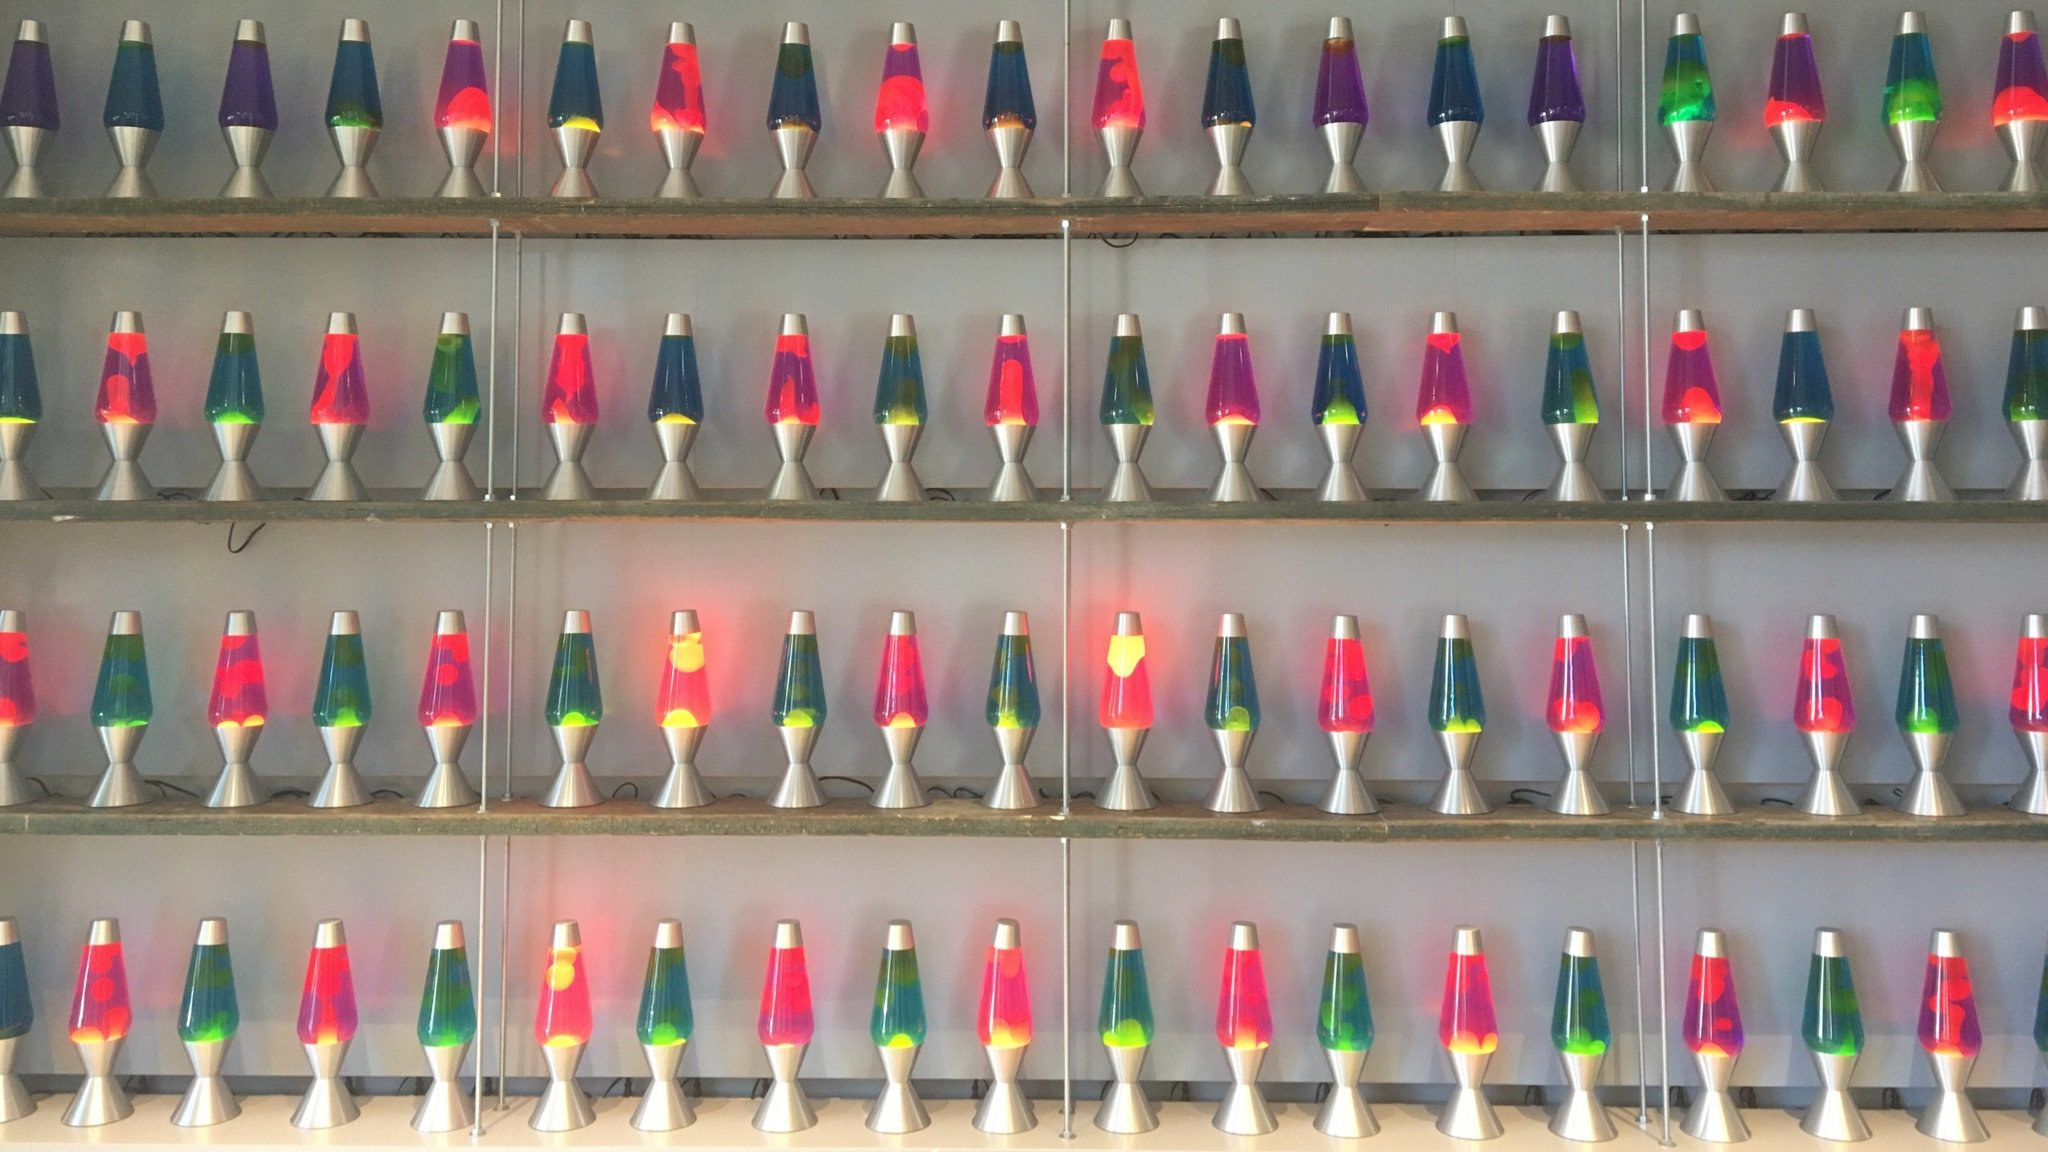
\includegraphics[scale = 0.2]{lava-lamps.jpg}
\end{figure}

\newpage 

\section{Definizioni utili per le sequenze casuali}
\footnote{Slide del prof | Generazione di variabili aleatorie | pag 1 \\ 
Appunti di Damiano | pag 1 \\ 
Slide | Generazione di variabili aleatorie | pag  1\\ 
Appunti | 2025-04-15 | pag 10
} 

Come scritto nel titolo della sezione, 
di seguito daremo delle definizioni per capire questo capitolo. \newline 

\newpage 

\subsection{Definizioni di sequenze}
\footnote{Slide del prof | Generazione di variabili aleatorie | pag 1\\ 
Appunti di Damiano | pag 1\\ 
Slide | Generazione di variabili aleatorie | pag  1 \\ 
Appunti | 2025-04-15 | pag 10
} 

\textbf{Sequenza binaria} 

Una sequenza $\underline{u}$ composta da $u_k$ elementi: 

{
    \Large 
    \begin{equation}
        \underline{u} = (u_k)
    \end{equation}
}

dove il singolo elemento $u_k$ appartiene ai valori dei numeri interi $\mathbb{Z}$ e può valere solo 0 o 1: 

{
    \Large 
    \begin{equation}
        u_k = \{0, 1\} \text{ per } u_k \in \mathbb{Z}_2
    \end{equation}
}

Talvolta la sequenza $\underline{u}$ può essere una sequenza binaria bipolare. \newline 

\textbf{Sequenza binaria bipolare}

Una sequenza $\underline{u}$ composta da $b_k$ elementi: 

{
    \Large 
    \begin{equation}
        \underline{u} = (b_k)
    \end{equation}

}

dove il singolo elemento $b_k$ può valere:

{
    \Large 
    \begin{equation}
        b_k = \{ -1, +1\}
    \end{equation}
}

dove se: 

{
    \Large 
    \begin{equation}
        \begin{cases}
            u_k = 0 \leftrightarrow b_k = -1 
            \\
            u_k = 1 \leftrightarrow b_k = + 1
        \end{cases}
    \end{equation}
}

\textbf{Sequenza binaria random}

Sequenza $\underline{u}$ dove ogni simbolo $u_k$ è equiprobabile: 

{
    \Large 
    \begin{equation}
        P(u_k = 0) = P (u_k = 1) = 0.5
    \end{equation}
}

e indipendente: 

{
    \Large 
    \begin{equation}
        P(u_k | u_i) = P(u_k) \text{ con } i \neq k
    \end{equation}
}

cioè $u_k$ non dipende da $u_i$. \newline 

\begin{tcolorbox}
    Nel seguito, salvo diversa indicazione, le sequenze si assumeranno di lunghezza infinita. \newline 

    Se una sequenza ha lunghezza finita N, la interpreteremo come una sequenza di lunghezza infinita e periodo N, ottenuta mediante ripetizione. \newline 

    In alte parole, all'interno di N i bit sono casuali, ma siccome si ripetono, la sequenza non è proprio random, cioè casuale. 
\end{tcolorbox}

\newpage 

\subsection{Definizioni di grandezze per le sequenze casuali}
\footnote{Slide del prof | Generazione di variabili aleatorie | pag 1\\ 
Appunti di Damiano | pag 1\\ 
Slide | Generazione di variabili aleatorie | pag  1\\ 
Appunti | 2025-04-15 | pag 10
} 

Definiamo ora le seguenti grandezze. \newline 

\textbf{Numero di simboli}

{
    \Large 
    \begin{equation}
        \begin{cases}
            d_0 = \text{ numero di simboli } u_k = 0 \text{ presenti in un periodo} 
            \\
            d_1 = \text{ numero di simboli } u_k = 1 \text{ presenti in un periodo} 
        \end{cases}
    \end{equation}
}


\textbf{Funzione di autocorrelazione}

Per funzione di autocorrelazione si intende la seguente formula R(i): 

{
    \Large 
    \begin{equation}
        R(i) = \sum_{k = 1}^{N} b_k \cdot b_{k+i} \text{ per } i = 0, 1, \dots, N-1
    \end{equation}
}

Per $i = 0$, R vale: 

{
    \Large 
    \begin{equation}
        R(0) = N
    \end{equation}
}

\begin{tcolorbox}
    Un breve ripasso da Tds: \\
    \url{https://github.com/ciccio25/appunti-teoria-dei-segnali/blob/main/Appunti%20Teoria%20dei%20segnali.pdf} \\
    Capitolo 13.2 - Medie di insieme - pag 153 \newline 

    Per le variabili aleatorie estratte dal processo sono calcolabili le medie di insieme. \newline 

Consideriamo il valore medio in $x_1$, che sarà dato da: 

{
    \Large 
    \begin{equation}
        <x_1> 
        = 
        \int_{- \infty}^{+\infty}
        x_1 f_1 (x_1; t_1) dx_1
    \end{equation}
}

Il momento congiunto di ordine (1, 1) delle variabili $x_1$ e $x_2$ si otterrà come: 

{
    \Large 
    \begin{equation}
        <x_1 x_2> 
        = 
        \int_{- \infty}^{+\infty}
        \int_{- \infty}^{+\infty}
        x_1 x_2 f_{12} (x_1, x_2; t_1, t_2) 
        dx_1
        dx_2
    \end{equation}
}

Il momento congiunto di ordine (1, 1), che rappresenta la correlazione tra le variabili aleatorie estratte $x_1$ e $x_2$; 
prende il nome di autocorrelazione statistica del processo e si indica con $R(t_1, t_2)$. \newline 

$\blacksquare$ \newline 

Invece, qui, siccome siamo nell'ambito dei numeri discreti, non useremo l'integrale, bensì una sommatoria. 
\end{tcolorbox}

\textbf{Corsa}

Una corsa, in inglese run, $C_L$ di lunghezza L è una sotto-sequenza di $\underline{u}$ costituita da L simboli consecutivi uguali. \newline 

In particolare, indicheremo con $C_L^{0}$ una corsa di L simboli consecutivi uguali a 0. \newline 

Indicheremo con $C_L^{0}$ una corsa di L simboli consecutivi uguali a 1. \newline 

Nel caso di sequenza di lunghezza finita (e dunque trattata come sequenza periodica), 
per attribuire correttamente il bit $u_0$ ad una corsa, si deve guardare $U_{N-1}$, cioè $U_{-1}$. \newline 

Si indica con $N_T$ il numero totale di corse nel periodo. \newline 

Si indica con $N_L$ il numero di corse $C_L$ nel periodo. \newline 

Si indica con $N_L^{0}$ il numeri corse $C_L^{0}$ nel periodo. \newline 

Si indica con $N_L^{1}$ il numeri corse $C_L^{1}$ nel periodo. \newline 

\newpage 

\subsection{Proprietà delle sequenze random}
\footnote{Slide del prof | Generazione di variabili aleatorie | pag 2 \\
Appunti di Damiano | pag 2 \\ 
Slide | Generazione di variabili aleatorie | pag  2\\ 
Appunti | 2025-04-15 | pag 10
} 

Asintoticamente, cioè per N molto grande, le sequenze random tendono ad avere queste tre proprietà: 

\begin{itemize}
    \item $d_0 = d_1$ (cioè il numero di simboli 0 ed 1 tende ad essere uguale) 
    \item $R(i) = 0$ per $i \neq 0$ (cioè il numero di coincidenze tende ad essere uguale al numero di discordanze, per ogni shift dato alla sequenza di partenza) 
    \item $N_L = \frac{N_T}{2^{L}}$ (cioè metà delle corse sono di lunghezza 1, un quarto 2, etc.) e $N_L^{1} = N_L^{0}$ (cioè le corse di una data lunghezza sono per metà corse di 1 e per metà corse di 0)
\end{itemize}

\newpage 

\section{Generazione di sequenze pseudo-random mediante LFSR}
\footnote{Slide del prof | Generazione di variabili aleatorie | pag 2 - 3\\
Appunti di Damiano | pag 2 - 3\\ 
Slide | Generazione di variabili aleatorie | pag  2 - 3\\ 
Appunti | 2025-04-15 | pag 10
} 

Siccome abbiamo a che fare con strumenti, come i microcontrollori, 
che sono degli strumenti progettati per svolgere dei compiti deterministici, 
purtroppo i dispositivi che abbiamo non riescono a generare delle sequenze veramente casuali. \newline 

Quindi, in pratica, ci si accontenta di generare sequenze pseudo-random, 
cioè con proprietà il più possibile simili a quelle delle sequenze random. \newline 

La generazione di buone sequenze pseudo-random può avvenire mediante una struttura 
che prende il nome di Linear Feedback Shift Register (oppure in acronimo LFSR). \newline 

\begin{tcolorbox}
    Perché, alla fine, il computer o qualsiasi microprocessore a basso livello, 
    è formato da registri.
\end{tcolorbox}

Un LFSR è un sistema a tempo discreto (generalmente temporizzato da un clock) 
costituito da R celle e R possibili connessioni. \newline 

Lo schema generale di un LFSR è il seguente: 

\begin{figure}[h]
    \centering
    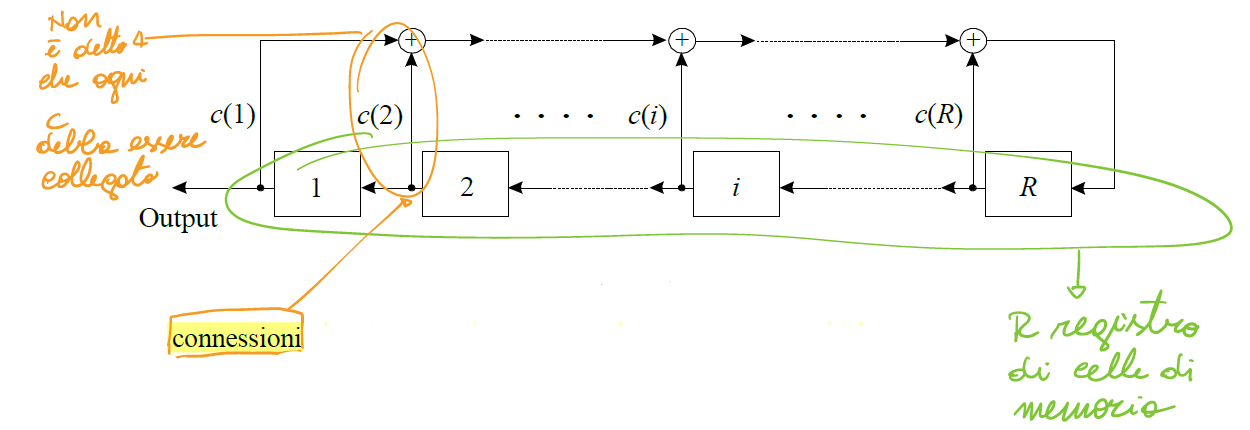
\includegraphics[scale = 0.7]{LFSR con note.PNG}
\end{figure}

Come scritto nelle note della figura, 
le connessioni sono numeri binari. \newline 

Ogni connessione i-esima si può scrivere come c(i) e può essere: 

{
    \Large 
    \begin{equation}
        c(i) = \{ 0, 1 \} \text{ per } c(i) \in \mathbb{Z}_2
    \end{equation}
}

Dal punto di vista circuitale: 

\begin{itemize}
    \item Se c(i) = 1, il collegamento è presente 
    \item Se c(i) = 0, il collegamento è assente
\end{itemize}

Le connessioni c(i) rimangono costanti nel tempo. \newline 

Il contenuto delle celle è binario e varia in corrispondenza di istanti discreti $t_k$: 

{
    \Large 
    \begin{equation}
        t_k = (k \cdot T)
    \end{equation}
}

(identificabili, ad esempio con il fronte di salita di un clock con periodo T). \newline 

\begin{tcolorbox}
    Circuitalmente un temporizzatore lo possiamo implementare in diverse maniere. \newline 

    Ti lascio un esempio sui timer 555: \newline 

    \url{https://youtu.be/oZzjmAbyyIQ?si=DRkYR_8KggpFJ2OU} \\
    How 555 timers Work - The Learning Circuit by element14presents \newline 

    Inoltre, qui spiegherò di seguito come funziona un LFSR per generare una sequenza pseudo-random in forma scritta, 
    ma grazie a questo video lo puoi visualizzare step-by-step anche graficamente e con un esempio in Python: \newline 

    \url{https://www.youtube.com/watch?v=Ks1pw1X22y4}\\
    Random Numbers with LFSR (Linear Feedback Shift Register) - Computerphile by Computerphile 
\end{tcolorbox}

Indicheremo il contenuto delle celle all'istante (discreto) k con i simboli: 

{
    \Large 
    \begin{equation}
        s(1)_{k}, \dots, s(R)_k \text{ con } s(i)_k \in \mathbb{Z}_2
    \end{equation}
}

All'istante k = 0, 
si assegna il valore iniziale alle R celle, 
ovvero si scelgono: 

{
    \Large 
    \begin{equation}
        \left[ s(1)_0, \dots, s(R)_0 \right]
    \end{equation}
}

\begin{tcolorbox}
    Ho messo le parentesi quadre come se la sequenza fosse 
    un vettore nel linguaggio di programmazione C
\end{tcolorbox}

Al generico istante k, 
il sistema si evolve nel seguente modo: 

\begin{enumerate}
    \item bit generato, si genera il bit, quindi: 
    {
        \Large 
        \begin{equation}
            u_k = s(1)_k
        \end{equation}
    }
    \item calcolo reazione, si calcola il bit di reazione: 
    {
        \Large 
        \begin{equation}
            x_k 
            =
            \sum_{i = 1}^{R}
            s(i)_k \cdot c(i)
        \end{equation}
    }
    Le somme ed i prodotti sono in $\mathbb{Z}_2$ (cioè possono essere solo 0 o 1): 
    in altre parole si fanno le somme modulo 2 utilizzando degli XOR
    \item calcolo stato futuro, avanzamento dello shift register e inserimento della reazione nell'ultima cella. \newline 
    Si ha:
    {
        \Large 
        \begin{equation}
            s(R)_{k+ 1} = x_k 
            \text{ }
            \forall j : 1 \le j \le R-1, s(j)_{k+1} = s(j+1)_k 
        \end{equation}
    }  
\end{enumerate}


\begin{tcolorbox}
    Per fare le somme modulo 2 si usano gli XOR. \newline 

    Un po' di materiale che ti può aiutare: \newline 

    \url{https://www.settorezero.com/wordpress/operazioni-algebriche-booleane-come-si-utilizzano-gli-operatori-and-or-xor-e-not-e-come-applicarli-ai-registri-ad-8-o-piu-bit/} \newline 

    \url{https://www.youtube.com/watch?v=VPw9vPN-3ac} \\
    XOR \& the Half Adder - Computerphile by Computerphile 
\end{tcolorbox}

Si dimostra, cioè non lo dimostriamo, che, scegliendo opportunamente le connessioni, 
si ottiene una sequenza $\underline{u}$: 

{
    \Large 
    \begin{equation}
        \underline{u} = (u_k)
    \end{equation}
}

con periodo massimo N: 

{
    \Large 
    \begin{equation}
        N = 2^{R} - 1
    \end{equation}
}

dove R sono il numero delle celle binarie. \newline 

Inoltre, si vuole ribadire che la scelta di avere un LFSR in cui l'evoluzione avviene da destra verso sinistra è puramente convenzionale. \newline 

\newpage 

\subsection{Proprietà di una sequenza con N massimo da LFSR}
\footnote{Slide del prof | Generazione di variabili aleatorie | pag 3 - 4 \\
Appunti di Damiano | pag 3 - 4 \\ 
Slide | Generazione di variabili aleatorie | pag  3 - 4\\ 
Appunti | 2025-04-15 | pag 10
} 

Una sequenza $\underline{u}$ di periodo massimo $N = 2^{R} - 1$, 
generata mediante LFSR, possiede le seguenti proprietà: 

\begin{itemize}
    \item $d_1 = d_0 + 1$
    \item $R(i) = - 1$ per ogni $i \neq 0$
    \item A partite dal valore di $N_T$, per qualunque lunghezza L si ha: 
    \begin{itemize}
        \item Per L compreso tra 1 e R, $N_L$ vale: $N_L = \frac{N_T}{2^{L}}$ e $N_L^{1} = N_L^{0}$
        \item Per L = R  $N_L$ vale: $N_L = N_L^{0} = 1$
        \item Per L = R, $N_L$ vale: $N_L = N_L^{1} = 1$
        \item Per $L > R$, $N_L$ vale: $N_L = 0$
    \end{itemize}
\end{itemize}

Confrontando le proprietà delle sequenze random con quelle random LFSR, 
notiamo che: 

\begin{itemize}
    \item $d_1 = d_0 + 1$, che è simile a $d_0 = d_1$ delle sequenze random 
    \item $R(i) = - 1$ per ogni $i \neq 0$, invece nelle sequenze random non è vera che la relazione deve valere per ogni valore diverso da zero 
    \item Per L compreso tra 1 e R, $N_L$ vale: $N_L = \frac{N_T}{2^{L}}$ e $N_L^{1} = N_L^{0}$, che è la stessa proprietà della sequenza random
\end{itemize}

\newpage 

\subsection{Collegamenti in un LFSR per avere periodo massimo}
\footnote{Slide del prof | Generazione di variabili aleatorie | pag 4 - 7 \\
Appunti di Damiano | pag 4 - 7 \\ 
Slide | Generazione di variabili aleatorie | pag  4 - 7\\ 
} 

Il contenuto iniziale delle R celle determina univocamente la sequenza $\underline{u}$ 
generata di periodo N. \newline 

Partire da una diversa configurazione delle R celle, 
corrisponde a generare una versione shiftata, nel tempo, della stessa sequenza. \newline 

Le connessioni che corrispondono ad un periodo massimo sono note e tabulate. \newline 

Dato un R, si possono utilizzare la seguente tabella per ricavare un periodo massimo: 

\begin{figure}[h]
    \centering
    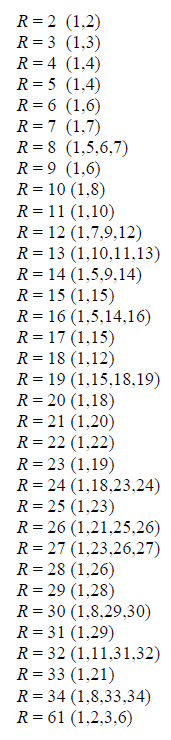
\includegraphics[scale = 1]{LFSR con periodo massimo tabella collegamenti.PNG}
\end{figure}

Va ribadito che le configurazioni sopra riportate non sono le uniche possibili e, 
a parità di valore di R, 
ne possono essere trovate altre equivalenti. \newline 

\newpage 

\section{Rappresentazione polinomiale di un LFSR}
\footnote{Slide del prof | Generazione di variabili aleatorie | pag 8 - 9 \\
Appunti di Damiano | pag 8 - 9
} 

Un aspetto molto interessante riguarda le modalità di rappresentazione dell'LFSR. \newline 

Se può rappresentare il LFSR con un polinomio h(x) di grado R, 
in cui saranno presenti soltanto le potenze della variabile formale x, 
rappresentative delle connessioni non nulle. \newline 

In particolare, visto che la potenza di grado R sarà sempre presente 
(sta a rappresentare la retroazione che determina l'aggiornamento dell'ultima cella dell'LFSR), 
se: 

{
    \Large 
    \begin{equation}
        c(i) = 1
    \end{equation}
}

comparirà, nella rappresentazione polinomiale, 
la potenza di $x^{i-1}$. \newline 

A titolo di esempio, si passerà dall'LFSR con i suoi elementi in vista grafica: 

\begin{figure}[h]
    \centering
    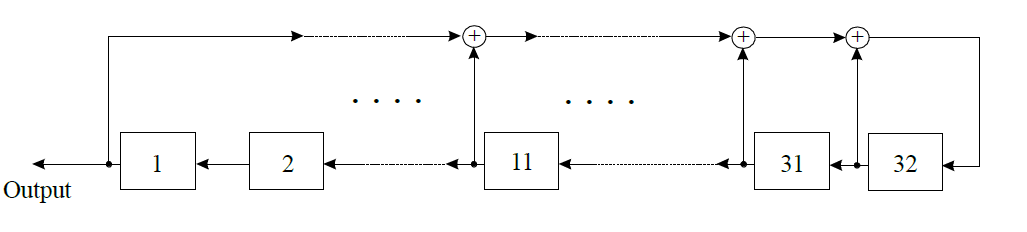
\includegraphics[scale = 0.7]{LFSR di esempio con rappresentazione polinomiale.png}
\end{figure}

a questa sua rappresentazione polinomiale: 

{
    \Large 
    \begin{equation}
        h(x) = x^{32} + x^{31} + x^{30} + x^{10} + 1
    \end{equation}
}

\begin{tcolorbox}
    Nel polinomio, è presente il termine +1, proprio perchè, 
    come si vede in figura, la cella dell'LFSR [1] ha un ramo di retroazione prima della scritta "Output".
\end{tcolorbox}

Essendo ora un polinomio, quindi una rappresentazione matematica, 
si può scegliere la base del polinomio, molto utile se abbiamo a che fare con polinomi molto grandi. \newline 

\begin{tcolorbox}
    A titolo di esempio, nell'esempio c'è scritto come convertire il polinomio h(x) da binario a ottale, 
    quindi un polinomio in base 8.
\end{tcolorbox}

Ricordando che la rappresentazione è una funzione biunivoca, 
anche il polinomio ha una sequenza di periodo massimo: 

{
    \Large 
    \begin{equation}
        N_{max} = 2^{R} - 1
    \end{equation}
}


\newpage 

\section{PSL di un LFSR}
\footnote{Slide del prof | Generazione di variabili aleatorie | pag 8 - 9\\
Appunti di Damiano | pag 8 - 9\\
Slide | Generazione di variabili aleatorie | pag  8 - 9 
} 

Può essere interessante osservare che, 
le proprietà delle sequenze di periodo massimo discusse in precedenza, 
vengono significativamente modificate nel caso in cui sia necessario troncare la sequenza. \newline 

Questa operazione va effettuato, ad esempio, nel caso in cui la sequenza generata debba adattarsi ad una struttura di frame pre-fissata. \newline 

\begin{tcolorbox}
    Si pensi ad avere una lunga stringa e la memoria in un microcontrollore è piccolissima. \newline 

    Dal punto di vista non tecnico, 
    è come avere un trasloco e mettere tutto quello che hai della vecchia casa in un'auto: 
    sarebbe impossibile. \newline 

    Ma se smonti ogni singolo componente e fai diversi viaggi con l'auto, 
    poi "traslocare" facilmente. 
\end{tcolorbox}

Emblematico, sotto questo aspetto, è il comportamento di un parametro fondamentale (che è molto utile nelle applicazioni che utilizzano sequenze pseudo-random) denominato Maximum Peak Slide Lobe, 
ed indicato con PSL. \newline 

Esso è definito come segue: 

{
	\Large 
	\begin{equation}
	PSL = \max_{i \neq 0} \abs{R(i)}
	\end{equation}

}

Nel caso di una sequenza di periodo massimo, 
con cioè:

{
    \Large 
    \begin{equation}
        N_{max} = 2^{R} - 1
    \end{equation}
}

allora possiamo dire che la sequenza ha PLS: 

{
    \Large 
    \begin{equation}
        PSL = 1
    \end{equation}
}

\newpage 

\section{Generazione di variabili casuali}
\footnote{Slide del prof | Generazione di variabili aleatorie | pag 10 \\
Appunti di Damiano | pag 10 \\ 
Slide | Generazione di variabili aleatorie | pag  10\\ 
Appunti | 2025-05-06 | pag 2
} 

Un problema che spesso si pone nella simulazione di un sistema di comunicazione è quello della generazione di campioni 
secondo una prefissata statistica. \newline 

L'esempio più importante, in questo caso, è quello dato dal rumore termico, 
i cui campioni, come noto, seguono una statistica gaussiana. \newline 

Per generare una variabile gaussiana, 
è preliminare necessario disporre di un algoritmo capace di generare campioni indipendenti di una variabile casuale 
uniformemente distribuita tra 0 e 1. \newline 

\newpage 

\subsection{Generazione di una variabile causale con distribuzione uniforme}
\footnote{Slide del prof | Generazione di variabili aleatorie | pag 10 \\
Appunti di Damiano | pag 10 \\ 
Slide | Generazione di variabili aleatorie | pag  10\\ 
Appunti | 2025-05-06 | pag 2
} 

Un buon algoritmo per la generazione della variabile uniforme è il seguente: 

\begin{enumerate}
    \item si fissa un valore iniziale $v_0$: 
    {
        \Large 
        \begin{equation}
            v_0 \neq 0
        \end{equation}
    }
    \item per generare un k-esimo campione $w_k$ si calcola prima $v_k$:
    {
        \Large 
        \begin{equation}
            v_k = a \cdot v_{k-1} \text{ mod } m
        \end{equation}
    }
    e poi $w_k$: 
    {
        \Large 
        \begin{equation}
            w_k = \frac{v_k}{m}
        \end{equation}
    }
\end{enumerate}

\begin{tcolorbox}
    Ricordo al volo che l'operatore mod restituisce il modulo tra $a \cdot v_{k-1}$ e m, 
    dove per modulo si può intendere anche il resto intero della divisione. \newline 
    
    Per ricavare $w_k$ si divide $v_k$ per m, in modo tale che $w_k$ venga normalizzato, 
    cioè rimanga tra un valore intero. 
\end{tcolorbox}

Se i valori di m e a sono scelti opportunamente, 
la sequenza $v_k$ ha periodo (m-1), 
cioè assume (m-1) valore diversi (tutti i numeri interi tra 1 e (m-1) compresi) 
in ordine pseudo-random, 
prima di ritornare al valore $v_0$. \newline 

La divisione per m, 
restituisce poi per un valore reale $w_k$ compreso tra 0 e 1 (esclusi). \newline 

Il resto della divisione non deve essere mai 0, altrimenti $v_k = 0$ e rimarrà 0 da quel momento in poi. \newline 

\newpage 

\subsection{Generazione di una variabile aleatoria secondo una assegnata statistica}
\footnote{Slide del prof | Generazione di variabili aleatorie | pag 14 \\
Appunti di Damiano | pag 14 \\ 
Slide | Generazione di variabili aleatorie | pag  14\\ 
Appunti | 2025-05-06 | pag 2 - 3
} 

Una volta che si dispone un generatore di variabile casuale uniforme, 
è possibile costruire semplici algoritmi per la generazione di una variabile casuale con distribuzione generica. \newline 

Indichiamo con V la variabile aleatoria uniformemente distribuita da 0 e 1. \newline 

La sua funzione di ripartizione (cioè la distribuzione di probabilità cumulativa), 
che esprime la probabilità che sia: 

{
    \Large 
    \begin{equation}
        V \le x
    \end{equation}
}

risulta: 

{
    \Large 
    \begin{equation}
        F_V (x)
        = 
        \begin{cases}
            0 \text{ per }  x < 0 
            \\
            x \text{ per } 0 \le x \le 1 
            \\
            1 \text{ per }  x > 1 
        \end{cases}
    \end{equation}
}

Consideriamo ora la distribuzione di probabilità cumulativa di un'altra variabile, 
la X, la cui densità di probabilità siamo interessati a simulare (cioè ad estrarre i relativi campioni). \newline 

Per definizione, sarà: 

{
    \Large 
    \begin{equation}
        F_X (a)
        = 
        \Pr \left[X \le A\right]
    \end{equation}
}

avendo indicato con $\Pr \left[X \le A\right]$ la probabilità dell'evento $X \le A$. \newline 

Poniamo ora la seguente trasformazione di variabile aleatoria: 

{
    \Large 
    \begin{equation}
        X = F_X^{-1} (V)
    \end{equation}
}

\begin{tcolorbox}
    Questa formula, è stata presentata nel corso senza dimostrazione
\end{tcolorbox}

che corrisponde a considerare l'inversa della funzione di ripartizione assegnata ad X e nel sostituire alla variabile indipendente la V 
(che, per ipotesi, è distribuita uniformemente). \newline 

\newpage 

\subsubsection{Dimostrazione dell'ammissibilità della trasformazione}
\footnote{Slide del prof | Generazione di variabili aleatorie | pag 14 - 15\\
Appunti di Damiano | pag 14 - 15\\ 
Slide | Generazione di variabili aleatorie | pag  14 - 15\\ 
Appunti | 2025-05-06 | pag 2 - 3
} 

\begin{tcolorbox}
    Dimostrazione utile solo se ti interessa, sennò saltala
\end{tcolorbox}

Di seguito la dimostrazione dell'ammissibilità della formula: 

{
    \Large 
    \begin{equation}
        X = F_X^{-1} (V)
    \end{equation}
}

Verifichiamo che, con il cambiamento di variabile proposta, 
la $\Pr \left[X \le A\right]$ restituisce proprio $F_X (a)$, 
e quindi il cambiamento di variabile è ammissibile e può essere utilizzato per generare i campioni di X a partire dai campioni di V. \newline 

In altre parole, si vuole fare la dimostrazione che $F_X^{-1} (V)$ ha le stesse proprietà di X. \newline 

Infatti: 

{
    \Large 
    \begin{equation}
        \Pr \left[X \le A\right] 
        = 
        \Pr \left[F_X^{-1} (V) \le a\right] 
    \end{equation}
}

Ora è evidente che: 

{
    \Large 
    \begin{equation}
        \begin{split}
            \Pr \left[F_X^{-1} (V) \le a\right] 
            &=
            \Pr
            \{ F_X \left[ F_X^{-1} (V)\right] \le F_X(a)\}
            \\
            &=
            \Pr \left[V \le F_X (a) \right] 
        \end{split}
    \end{equation}
}

Per definizione risulta: 

{
    \Large 
    \begin{equation}
       \Pr \left[V \le F_X (a) \right] 
       = 
       F_V \left[ F_X (a) \right]  
    \end{equation}
}

e poiché: 

{
    \Large 
    \begin{equation}
        F_V (x) = x \text{ per } 0 \le x \le 1
    \end{equation}
}

ed effettivamente risulta: 

{
    \Large 
    \begin{equation}
        0 \le F_X (a) \le 1
    \end{equation}
}

si ha infinite: 

{
    \Large 
    \begin{equation}
         \Pr \left[V \le F_X (a) \right] 
         = 
         F_X (a)
    \end{equation}
}

il che dimostra la tesi. \newline 

\newpage 

\subsubsection{Metodo di trasformazione}
\footnote{Slide del prof | Generazione di variabili aleatorie | pag 15 \\
Appunti di Damiano | pag 15 \\ 
Slide | Generazione di variabili aleatorie | pag  15\\ 
Appunti | 2025-05-06 | pag 3
} 

Sulla base della dimostrazione precedente, 
l'algoritmo per generare i campioni di una generica variabile aleatoria X, 
di cui si conosca in forma esplicita la distribuzione di probabilità cumulativa 
o la funzione di densità di probabilità 
(visto che una è la derivata dell'altra), 
può essere sintetizzato con il "metodo di trasformazione". \newline 

Di seguito l'algoritmo step-by-step: 

\begin{enumerate}
    \item Si inverte la funzione di ripartizione assegnata trovando $F_X^{-1} (x)$ 
    \item Si genera una variabile aleatoria uniforme $V \in [0, 1]$ 
    \item Si genera un campione (in inglese prende il nome di variate) della variabile X attraverso la trasformazione $X = F_X^{-1} (V)$
\end{enumerate}

\newpage 

\subsubsection{Algoritmo Box-Muller}
\footnote{Slide del prof | Generazione di variabili aleatorie | pag 20 \\
Appunti di Damiano | pag 20 \\
Slide | Generazione di variabili aleatorie | pag  20\\  
Appunti | 2025-05-06 | pag 4
} 

Quando si hanno variates della variabile gaussiana va sotto il nome di Algoritmo (o Metodo) di Box-Muller. \newline 

Da un punto di vista operativo, questi sono gli step dell'algoritmo: 

\begin{enumerate}
    \item Si generano le variates di due variabili uniformi tra -1 e +1 
    \item Si costituisce le variate della variabile uniforme tra 0 e 1, sommando i quadrati delle variates trovate al passo precedente 
    \item Si verifica che la variate generata non sia maggiore di 1, sennò si ritorna al primo step, altrimenti si procede 
    \item Si calcolano le variates della variabile gaussiana utilizzando le varietes del primo e del secondo passaggio
\end{enumerate}


\newpage 
